%%%%%%%%%%%%%%%%%%%%% restrictions.tex %%%%%%%%%%%%%%%%%%%%%%%%%%%%%%
%
% sample chapter
%
% Use this file as a template for your own input.
%
%%%%%%%%%%%%%%%%%%%%%%%% Springer-Verlag %%%%%%%%%%%%%%%%%%%%%%%%%%

\section{Ficheiros de Dados}
\label{data:1}

Os ficheiros de dados são simples ficheiros de texto (\textit{.txt}), que em cada linha têm os dígitos de cada face.
As faces encontram-se pela seguinte ordem: Topo, Baixo, Frente, Trás, Esquerda e por fim Direita.

De seguida encontra-se um exemplo deste ficheiro com os valores do problema original:

\begin{f_exemplo}[H]
\begin{verbatim}

356735869637537564374649
343574954363596738547975
353748635975458485676439
349576573795398457964379
357863653739359498735895
348765738453874583769785
\end{verbatim}
\caption{Problema original do turn12, com 24 dígitos por face:}
\end{f_exemplo}



\section{Variáveis de Decisão}
\label{restr:1}

As variáveis de decisão usadas na solução foram as rotações que podiam ser feitas em cada face do cubo.\\
Estas rotações têm um domínio compreendido entre 1 e o número de dígitos de cada face.

\section{Restrições}
\label{restr:2}

Independentemente do número de dígitos em cada face, verificou-se que as restrições seriam sempre as mesmas: a soma dos dígitos dos cantos onde cada face se toca, teria de ser 12.\\

De forma a fazer a sua implementação, foi utilizado no \textit{SICStus Prolog} a biblioteca de restrições para o conjunto dos domínios finitos \textit{clp(FD)}, onde foram definidas variáveis que seriam preenchidas com os valores dos cantos tendo em conta a rotação aplicada sobre cada face, e restringidas de forma que a soma onde todas se tocam ser obrigatoriamente 12.

\section{Função de Avaliação}
\label{restr:3}

A predicados de avaliação chamam-se \textit{turn12}. Existem três implementados (com o mesmo nome) na solução, mas o principal aceita como parâmetros de entrada as 6 faces do cubo, que deverão ser cada um uma lista numérica de dígitos. Se for encontrada uma solução, são definidas como parâmetros de saída as rotações respectivas a cada face. São também definidos e agrupados 4 a 4 os valores da solução. Este predicado tem como objectivo apenas retornar a primeira solução encontrada.\\
Outro predicado, com o mesmo nome, tem como parâmetro de entrada, a localização do ficheiro com a informação de cada face, e só termina ate imprimir todas as soluções que um problema pode ter.
Por fim, existe ainda uma última função que não aceita qualquer parâmetro, e que chama o predicado anteriormente descrito, com um ficheiro numa localização predefinida.


\section{Estratégia de Pesquisa}
\label{rest:4}

A estratégia de pesquisa tem como base começar por rodar cada face até encontrar uma solução.
De forma a optimizar a resolução do problema, o algoritmo começa apenas com duas faces, e tenta encontrar através do predicado de etiquetagem \textit{labeling}, uma rotação para cada que consiga somar o valor 12 onde ambas se tocam.
Quando encontrada, é passada para outra face do cubo, e com recurso a outro predicado de etiquetagem é tentado encontrar uma rotação para esta última que consiga satisfazer as mesmas restrições para os cantos em comum com as duas faces anteriores. É seguida sempre a mesma estratégia para as restantes faces, fazendo que a complexidade algorítmica seja sempre o mais inferior possível.
A razão para a utilização de vários predicados de etiquetagem deve-se ao facto de ser utilizado um predicado auxiliar (\textit{shifted\_face}) que preenche as variáveis utilizadas para testar as restrições com base na rotação correspondente, e tendo-se verificado que quando utilizado um único predicado para o mesmo efeito, o \textit{shifted\_face} era chamado desnecessariamente, mesmo para as faces em que a rotação se mantinha igual e que não tinham originado a falha.
Após isolados, o predicado só passou a ser chamado para a face do respectivo labeling, e evitando um varrimento contínuo e dispendioso nas várias listas de dígitos de cada face.

\section{Visualização da Solução}
\label{rest:5}

A visualização da solução é feita através do predicado \textit{project\_cube}.
Este predicado aceita faz uma projecção do cubo 3D em 2D, e tem como parâmetros de entrada os valores da solução encontrada pelo algorítmo de procura. Estes parâmetros são passados em grupos de 4, os cantos de cada face pela seguinte ordem: canto superior da face, canto direito da face, canto de baixo e canto esquerdo. Sendo a ordem de passagem das faces a seguinte: Topo,Trás, Direita, Esquerda, Frente, Baixo.

\begin{figure}[h!]
\begin{center}
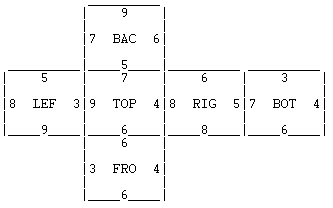
\includegraphics[scale=0.8]{resol.png}
\caption{Impressão da solução do problema original do turn12.}
\label{fig:1}
\end{center}
\end{figure}


%
